\chapter{Evaluation}\label{chap:eval}

A user study was conducted to evaluate the efficiency, effectiveness, and user-friendliness of Replico. The main goal was to determine how easily users could communicate points of interest within the virtual environment using Replico. Secondary goals included assessing ease of use and overall user experience. The study aimed to answer four key research questions:

\begin{itemize}
    \item \textbf{RQ1}: How efficiently can users create a point of interest on a given object?
    \item \textbf{RQ2}: How effectively does Replico notify users when a point of interest is created?
    \item \textbf{RQ3}: How useful is the world-in-miniature metaphor for communicating points of interest? How useful is the representation of user locations on the replica for understanding intent?
    \item \textbf{RQ4}: How user-friendly is Replico, and how much physical effort is required to use it? 
\end{itemize}

\section{Setup}

    % TODO: get computer specs

    The user study was conducted at FEUP, in the GIG laboratory in room I220. The setup included two VR-ready computers connected to a local network. Each computer had an HTC Vive Pro 2 headset and a VR controller for table tracking. Two touch surfaces -- a 32-inch infrared frame and a 47-inch capacitive Displax Skin Ultra touchscreen -- were placed on opposite tables within the central VR play space. Participants, in pairs, were seated in front of each touch surface with their backs facing each other, as shown in Figure \ref{fig:eval_setup}.

    \begin{figure}[h]
        \centering
        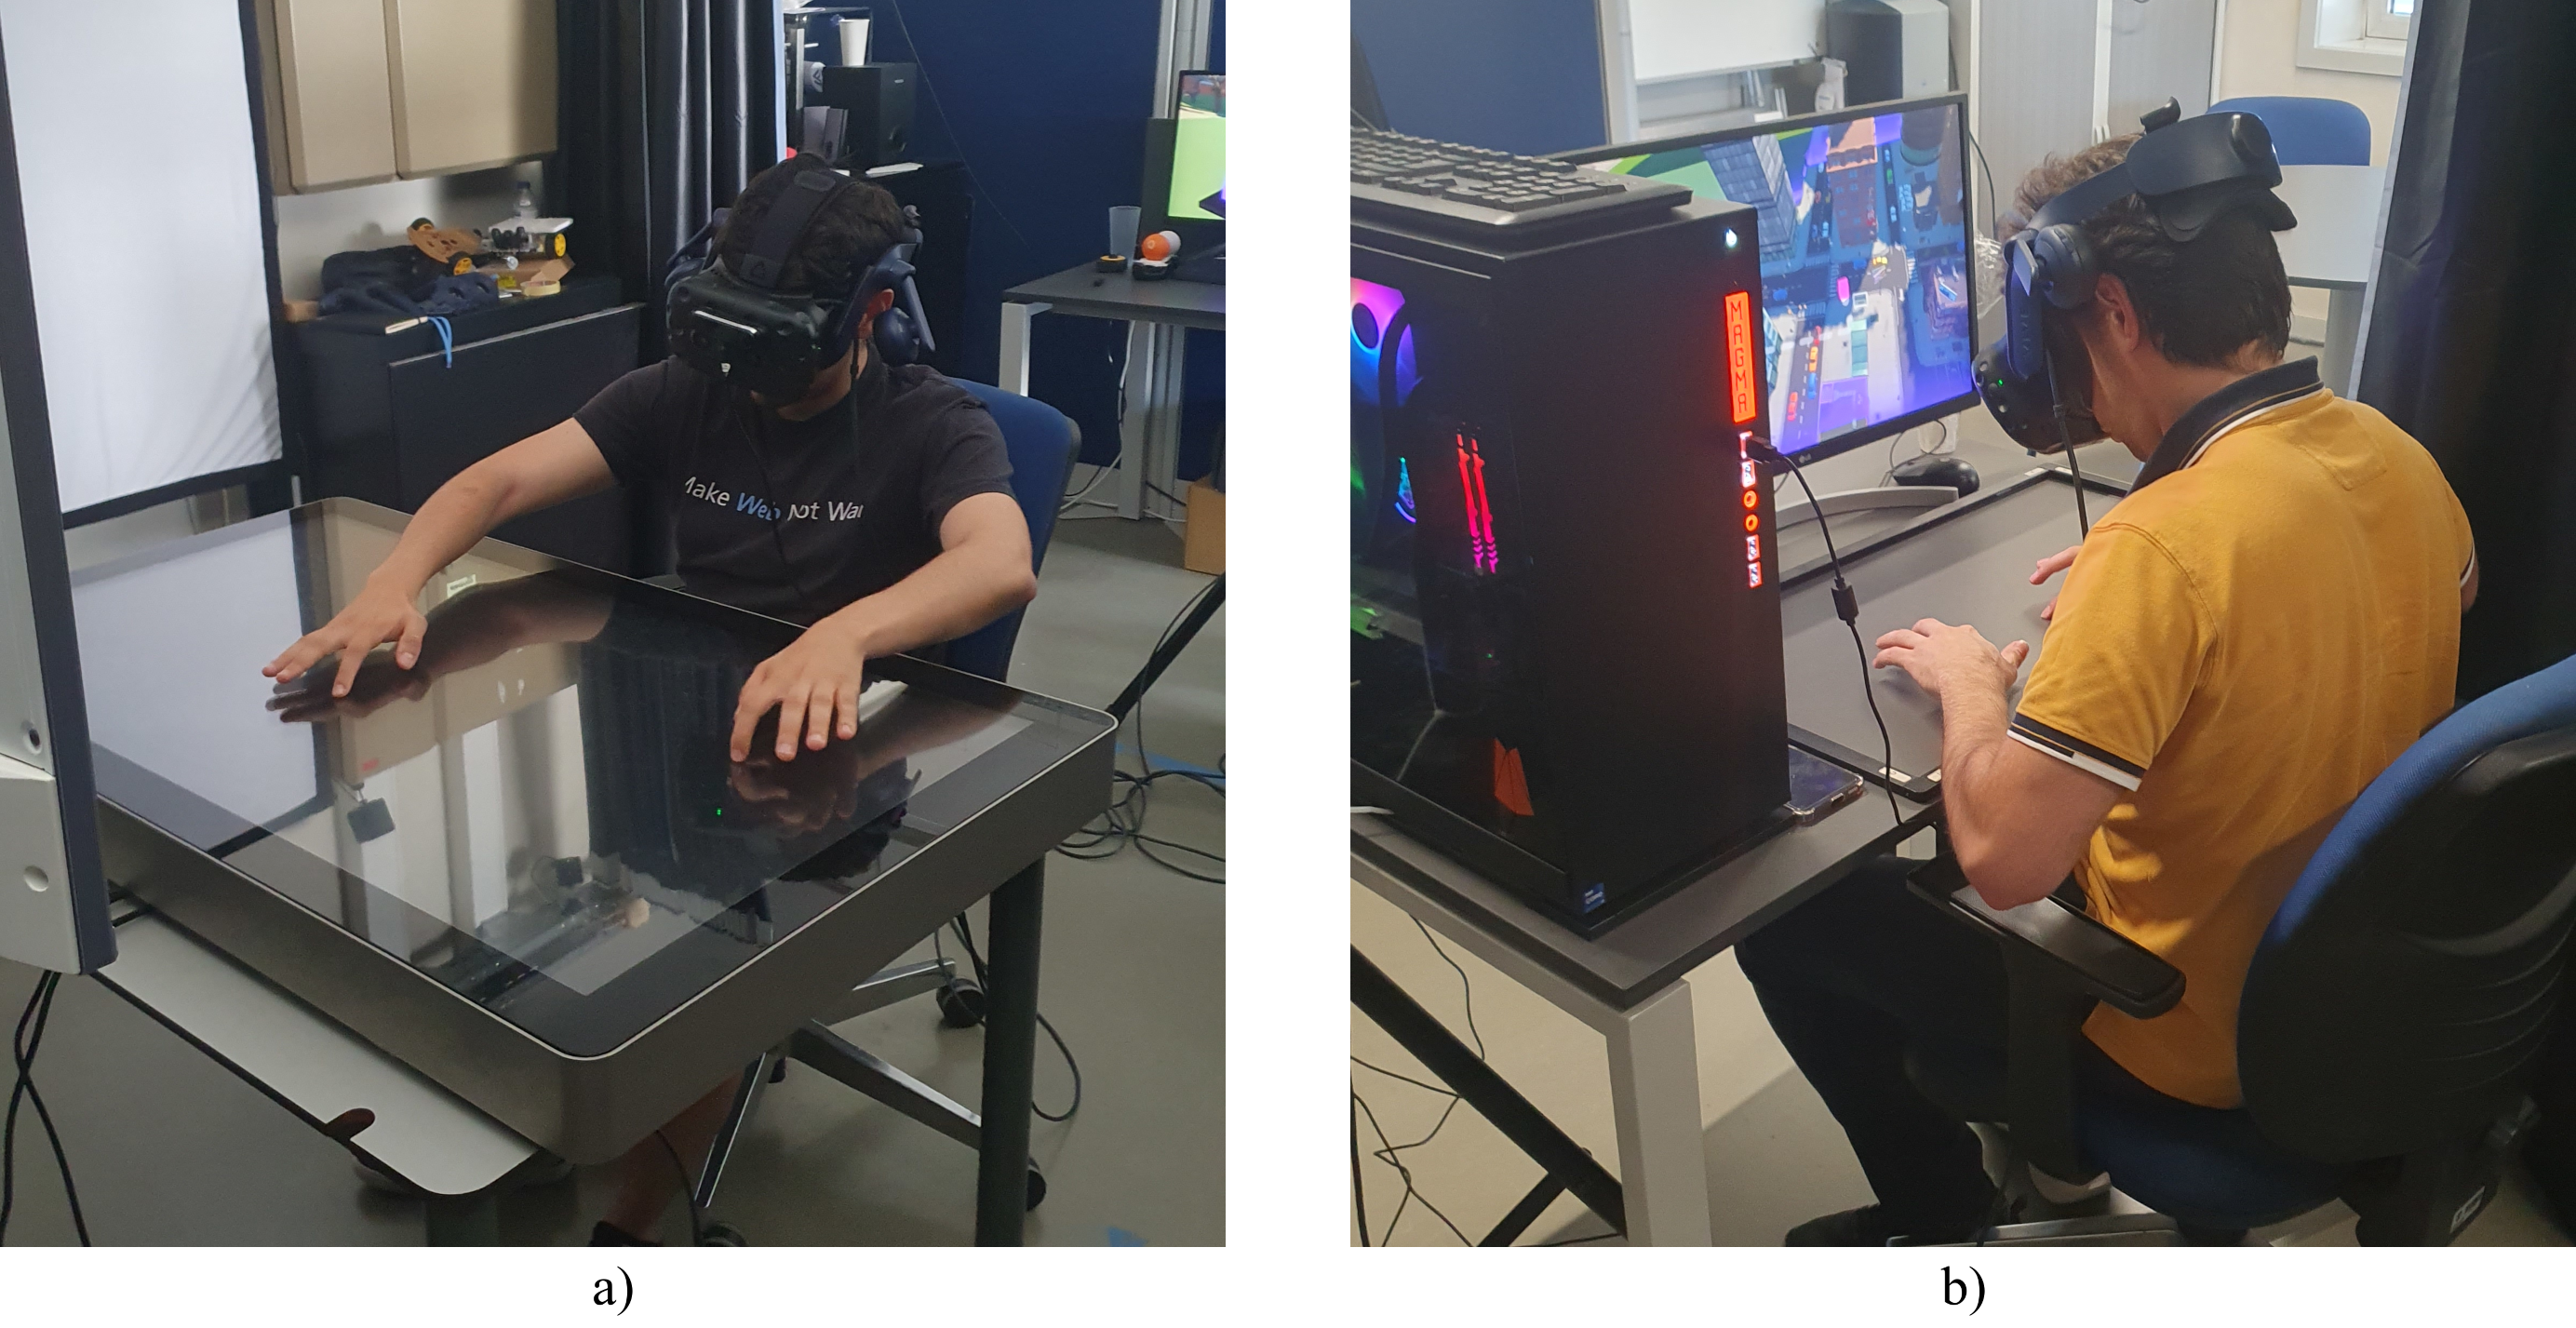
\includegraphics[width=1\linewidth]{figures/setup.png}
        \caption{Setup for the user study. In image (a) one participant is seated in front of the Displax Skin Ultra. In image (b) the participant is seated in front of the infrared touch frame.}
        \label{fig:eval_setup}
    \end{figure}

    One computer served as the host, while the other connected as a client. The setup process involved a starting screen where the moderator could select the IP address of the host computer. The roles of each computer did not change throughout the study, to simplify the setup process and avoid confusion.

\section{Methodology}

    The study was conducted in pairs, with initial tasks performed individually and later tasks performed collaboratively. It consisted of three main parts: an introduction, a training session, and the main tasks. Each session lasted approximately 60 minutes. At the conclusion of the study, participants received a chocolate bar as a token of appreciation.

    Before the study began, participants received a brief introduction to the study's purpose and the Replico system. They then completed a consent form and a profiling questionnaire. Following this, they watched a video presentation explaining Replico's features, usage, and the tasks they would perform.

    During the training session, participants familiarized themselves with the system by experimenting with all of Replico's features. Once comfortable with the solo interactions, a set of points of interest and a simulated player were added to the environment, allowing users to practice acknowledging points of interest and joining the other user's table. After becoming comfortable with these interactions, they proceeded to the main tasks.

    The main tasks were performed using two different 3D models: a city and the Perseverance rover, described in Section \ref{sec:test_scenarios}. To avoid bias, the order in which the models were used alternated between pairs. These tasks aimed to assess the efficiency and effectiveness of Replico's features, as described in Section \ref{sec:tasks}. Metrics for each task were collected as detailed in Section \ref{sec:evaluation_metrics}. Between each test scenario, participants completed a questionnaire on the tasks they performed, described in Section \ref{sec:qualitative_data}.


    \subsection{Test Scenarios} \label{sec:test_scenarios}

        Three scenarios were used during the study, two of which were used for the main tasks, as shown in Figure \ref{fig:test_scenarios}. The first scenario involved a small dungeon tavern, which was used for training. It was built using the free version of KayKit Dungeon Remastered Pack on itch.io\footnote{\url{https://kaylousberg.itch.io/kaykit-dungeon-remastered}}, and the Modular Asset Staging Tool (MAST) for Unity\footnote{\url{https://fertile-soil-productions.itch.io/mast}}. The second scenario was a city, from the POLYGON City Pack on the Unity Asset Store\footnote{\url{https://assetstore.unity.com/packages/3d/environments/urban/polygon-city-low-poly-3d-art-by-synty-95214}}, obtained with Unity's student plan. The third scenario was the Perseverance rover, obtained from NASA's 3D model repository\footnote{\url{https://nasa3d.arc.nasa.gov/detail/perseverance-glb}}, and the surrounding environment was created using Unity's terrain tools, and a tinted sand texture\footnote{\url{https://polyhaven.com/a/sand_01}}.


        \begin{figure}[h]
            \centering
            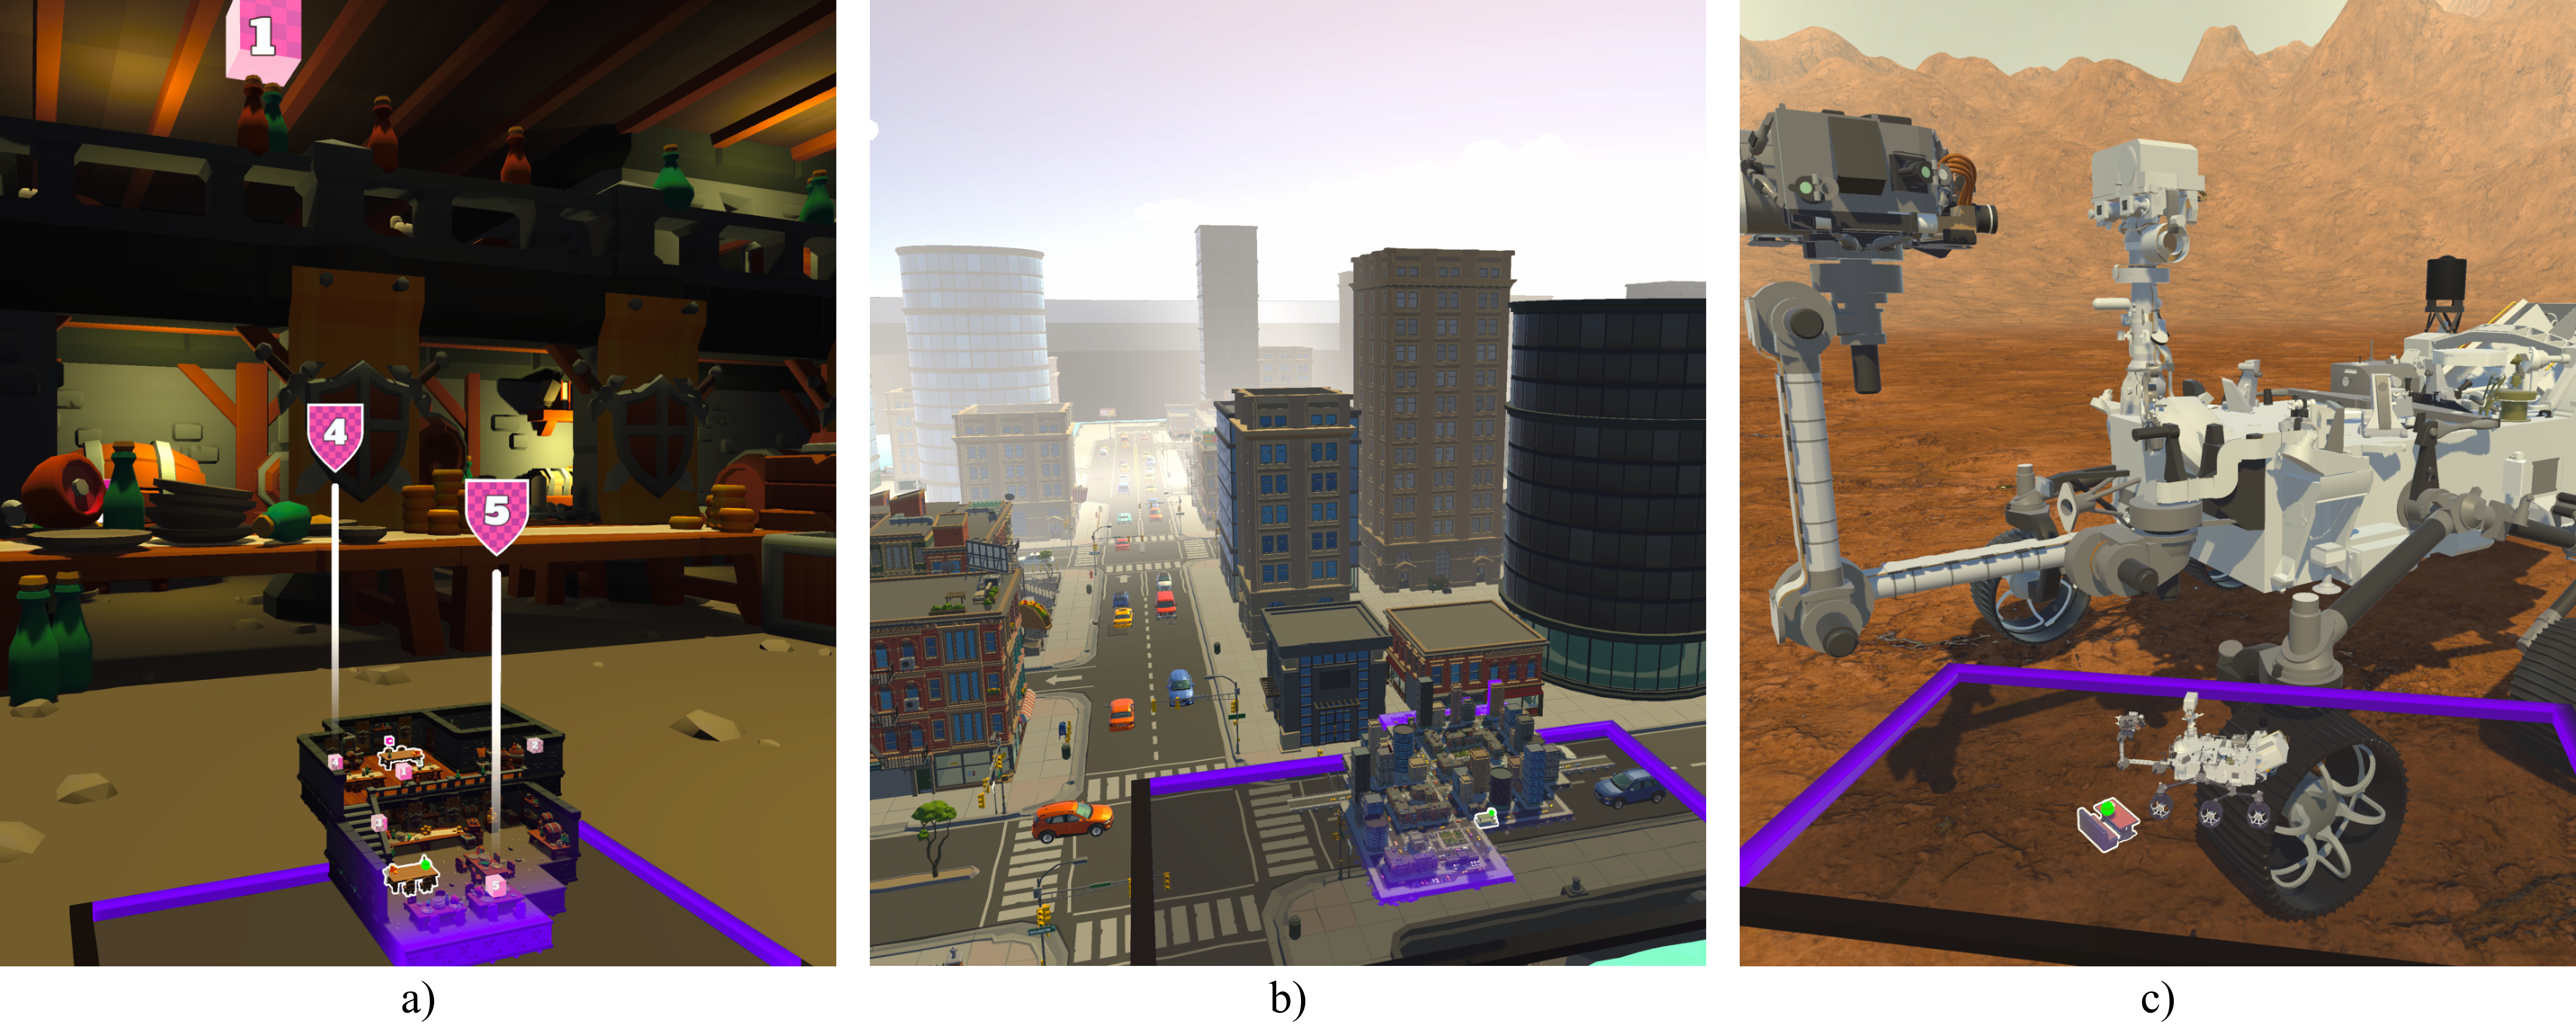
\includegraphics[width=1\linewidth]{figures/test_scenarios.png}
            \caption{The three test scenarios used in the user study. From left to right: the dungeon tavern, the city, and the Perseverance rover.}
            \label{fig:test_scenarios}
        \end{figure}

        % explain why these scenarios were chosen
        % and why there even are two scenarios
            % experiment how well the approach works with different 3D models:
                % a large one where the user can't see the whole model at once, and can be a part of the model, or can walk inside it
                % a small one where the user can see the whole model at once, and can't be a part of the model


    \subsection{Tasks} \label{sec:tasks}

    \subsection{Metrics} \label{sec:evaluation_metrics}

    \subsection{Qualitative Data} \label{sec:qualitative_data}

% do speak about how the frame being too sensitive to resting arms impacted the results